\documentclass[UTF8]{ctexart}

%固定图片位置
\usepackage{float}

%插入超链接
\usepackage{url}

\usepackage{tikz,mathpazo}
\usetikzlibrary{shapes.geometric, arrows}
\usetikzlibrary{calc}


\usepackage{listings}
%插入代码的配置
\definecolor{CPPLight}  {HTML} {686868}
\definecolor{CPPSteel}  {HTML} {888888}
\definecolor{CPPDark}   {HTML} {262626}
\definecolor{CPPBlue}   {HTML} {4172A3}
\definecolor{CPPGreen}  {HTML} {487818}
\definecolor{CPPBrown}  {HTML} {A07040}
\definecolor{CPPRed}    {HTML} {AD4D3A}
\definecolor{CPPViolet} {HTML} {7040A0}
\definecolor{CPPGray}  {HTML} {B8B8B8}
\lstset{
	language=Python,                                     % 设置语言
    columns=fixed,    
    breaklines = true,   
    basicstyle=\small ,
    numbers=left,                                        % 在左侧显示行号
    %frame=none,                                          % 不显示背景边框
    backgroundcolor=\color[RGB]{245,245,244},            % 设定背景颜色
    keywordstyle=\color[RGB]{40,40,255},                 % 设定关键字颜色
    numberstyle=\tiny\color{darkgray},           % 设定行号格式
    %commentstyle=\it\color[RGB]{0,96,96},                % 设置代码注释的格式
    stringstyle=\rmfamily\slshape\color[RGB]{128,0,0},   % 设置字符串格式
    showstringspaces=false,                              % 不显示字符串中的空格                           
    %morekeywords={True,alignas,continute,friend,register,true,alignof,decltype,goto,
    %reinterpret_cast,try,asm,defult,if,return,typedef,auto,delete,inline,short,
    %typeid,bool,do,int,signed,typename,break,double,long,sizeof,union,case,
    %dynamic_cast,mutable,static,unsigned,catch,else,namespace,static_assert,using,
    %char,enum,new,static_cast,virtual,char16_t,char32_t,explict,noexcept,struct,
    %void,export,nullptr,switch,volatile,class,extern,operator,template,wchar_t,
    %const,false,private,this,while,constexpr,float,protected,thread_local,
    %const_cast,for,public,throw,std,rand},
    emph={access,and,break,class,continue,def,del,elif ,else,%
	except,exec,finally,for,from,global,if,import,in,i s,%
	lambda,not,or,pass,print,raise,return,try,while},
    emphstyle=\color{CPPViolet}, 
    emph={[2]True, False, None, self},
	emphstyle=[2]\color{green},
	emph={[3]from, import, as},
	emphstyle=[3]\color{blue},
	upquote=true,
	morecomment=[s]{"""}{"""},
	commentstyle=\color{orange}\slshape,
	emph={[4]1, 2, 3, 4, 5, 6, 7, 8, 9, 0},
	emphstyle=[4]\color{red},
	emph={[5]numpy, np, plt},
	emphstyle=[5]\color{red},
	literate=*{:}{{\textcolor{blue}:}}{1}%
	{=}{{\textcolor{blue}=}}{1}%
	{-}{{\textcolor{blue}-}}{1}%
	{+}{{\textcolor{blue}+}}{1}%
	{*}{{\textcolor{blue}*}}{1}%
	{!}{{\textcolor{blue}!}}{1}%
	{(}{{\textcolor{blue}(}}{1}%
	{)}{{\textcolor{blue})}}{1}%
	{[}{{\textcolor{blue}[}}{1}%
	{]}{{\textcolor{blue}]}}{1}%
	{<}{{\textcolor{blue}<}}{1}%
	{>}{{\textcolor{blue}>}}{1},%
	framexleftmargin=0.1mm, framextopmargin=0.1mm, frame=shadowbox, rulesepcolor=\color{black},
}



\usepackage{geometry}
\geometry{left=2cm, right=2cm, top=1.2cm, bottom=1.2cm}

%得到引用的标题内容
\usepackage{nameref} 

%添加首行缩进,两个字符
\usepackage{indentfirst}
\setlength{\parindent}{2em}

%多行公式一个编号
\usepackage{amsmath}

%文献引用,标准类型为plain
%\usepackage[hyperref=true,backend=biber,sorting=none,backref=true]{biblatex}
%\addbibresource{ref.bib}
\bibliographystyle{plain}
\usepackage{cite}

\pagestyle{plain}

%跨页表格
\usepackage{multirow}
\usepackage{longtable,booktabs}
\usepackage{supertabular}
\usepackage{makecell}

%调整itemize等的间距
\usepackage{enumitem}


\usepackage{graphicx}
\usepackage{subfigure}

%超链接
\usepackage[linkcolor=yellow,citecolor=red,backref=page,hyperfootnotes=true]{hyperref}
\hypersetup{
bookmarks=true,
colorlinks=true,
linkcolor=black
}
\usepackage{tabularx} %This package must be placed after package {hyperref}, otherwise footnote marks are NOT treated as hyperlinks.


%引入了一些改进的数学环境,如align
\usepackage{amsmath}

\title{数据结构:Broadcast}
\author{姓名:鲁国锐 \protect\newline
\and 学号:17020021031 \\
\and 专业:电子信息科学与技术}


\begin{document}
	\maketitle
	\renewcommand{\contentsname}{Contents}
	\tableofcontents
	\newpage
	
	\hypersetup{
	bookmarks=true,
	colorlinks=true,
	linkcolor=red,
	urlcolor=blue
	}
	\section{问题分析}
	\subsection{题目描述}
	\indent 某广播公司要在一个地区架设无线广播发射装置。该地区共有$n$个小镇,每个小镇都要安装一台发射机并播放各自的节目。

	\indent 不过,该公司只获得了$FM104.2$和$FM98.6$两个波段的授权,而使用同一波段的发射机会互相干扰。已知每台发射机的信号覆盖范围是以它为圆心,$20km$为半径的圆形区域,因此,如果距离小于$20km$的两个小镇使用同样的波段,那么它们就会由于波段干扰而无法正常收听节目。现在给出这些距离小于$20km$的小镇列表,试判断该公司能否使得整个地区的居民正常听到广播节目。

     \subsection{输入}
     \indent 第一行为两个整数$n$,$m$,分别为小镇的个数以及接下来小于$20km$的小镇对的数目。 接下来的$m$行,每行$2$个整数,表示两个小镇的距离小于$20km$(编号从$1$开始)。
     
     \subsection{输出}
     \indent 如果能够满足要求,输出$1$,否则输出$-1$。

	\subsection{问题分析}\label{analysis}
	\indent 我们可以分三种情况分析:
	\begin{enumerate}[leftmargin=50pt]
	\item 距离小于$20$千米的村庄连成一个边数为偶数的多边形且对角线不连通,此时我们会发现只需要令相邻村庄交替使用两个波段就可以避免冲突;
	\item 距离小于$20$千米的村庄连成一个边数为奇数的多边形且对角线不连通,此时一定会产生冲突;
	\item 距离小于$20$千米的村庄连成一个多边形且对角线连通,此时对角线会将多边形划分成多个更小的对角线不连通的多边形,此时我们把问题化归为了对第一第二中情况的讨论。
	\end{enumerate}
	
	\indent 综合以上三种情况我们发现,判断是否会产生冲突问题就被转化成了寻找图中是否存在边数为奇数的多边形的问题。
	
	

	
	\section{解决方案}
		
		\indent 虽然我们已经分析出了是否会产生冲突的充分必要条件,但是直接用递归来穷举所有最小闭环成本太高。所以\ref{analysis}节中的结论虽然简明但不实用。
		
		\indent 所以这里我们转换思路,采取广度优先搜索的方法。我们先找到一个非孤立的村庄,然后以它为起点进行广度优先搜索。在搜索的过程中,要确保跟当前村庄直接连接的为被发现的村庄使用的波段跟自己不同。这里我们用一个名为$status$的$vector$来记录个村庄的状态:$0$表示为发现;$1$、$-1$分别表示使用的两种波段。
		
		\indent 用这种方法判断是否会产生冲突的条件就是对每一个访问到的村庄,遍历其所有邻接村庄,只要找到一个波段跟当前村庄相同的,就说明一定会产生冲突;若成功对这个连通域进行了一次遍历,则说明在该连通域中不会产生冲突。\textbf{注意只是在该连通域中不会产生冲突,可能还存在着其它连通域,我们需要对它们一一进行判断}。
	
	\section{算法设计}

\begin{figure}[H]
	\centering 
	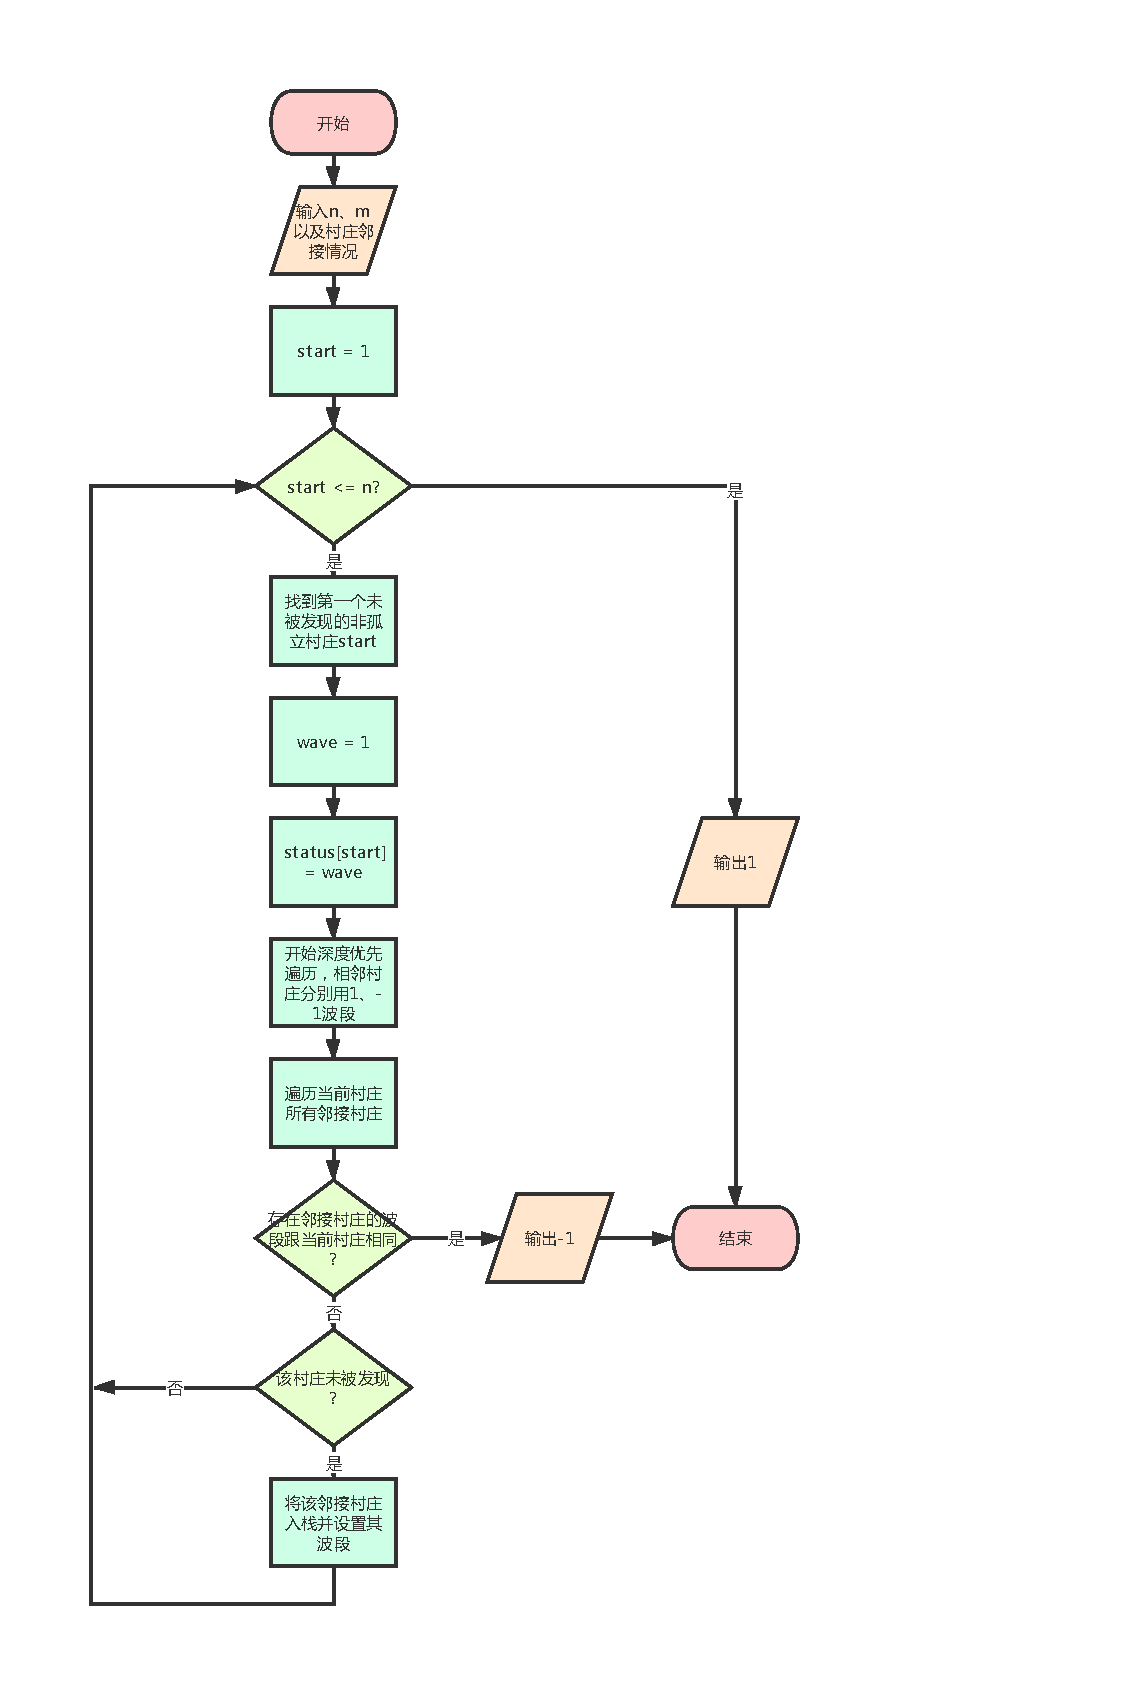
\includegraphics[scale=0.8]{broadcast_main.pdf} 
	\caption{$main$函数流程图} 
	\label{main}
\end{figure}




	\section{编程实现\protect \footnotemark[1]}
	\footnotetext[1]{完整的代码:\url{https://github.com/chenfeng123456/CourseInOUC/tree/master/algorithm/pa3_sourcecode}}

	\begin{lstlisting}[language=C++,caption={boradcast.cpp},label={broadcast.cpp}]
#include <iostream>
#include <vector>
#include <queue>
using namespace std;


bool linked(vector< vector<int> > &towns, int i)
{
    for (int j = 1; j < towns[i].size(); j++)
    {
        if (towns[i][j])
            return true;
    }
    return false;
}

int main()
{
    int n, m;
    cin >> n >> m;

    // 0 -> undiscovered; 1, -1 -> wave band
    vector<int> status(n+1, 0);
    vector< vector<int> > towns(n+1, vector<int>(n+1, 0));

    for (int i = 0; i < m; i++)
    {
        //cout << towns.size() << "  " << towns[0].size() << endl;
        int t1, t2;
        cin >> t1 >> t2;
        towns[t1][t2] = 1;
        towns[t2][t1] = 1;
    }

    int start = 1;
    while(start <= n)
    {
	    //find the first town which is not isolated
	    for (; start <= n; start++)
	    {
		    if (linked(towns, start) && (status[start] == 0))
            {
                //cout << status[start] << endl;
                break;
            }
        }
	    if (start > n)
	    {
		    //cout << "start > n" << endl;
		    cout << 1 << endl;
		    return 0;
	    }
	    //cout << "start = " << start << endl;

	    int wave = 1;
	    status[start] = wave;
	    queue<int> q;
	    q.push(start);
	    while (!q.empty())
	    {
		    wave = -wave;
		    int v = q.front();
		    q.pop();
		//cout << endl << "v = " << v << endl;

		    for (int u = 1; u <= n; u++)
		    {
		        if (towns[v][u])
		        {
		            if (status[u] == status[v])
		            {
		                //cout << "status[" << u << "] = " << status[u] << endl;
		                //cout << "status[" << v << "] = " << status[v] << endl;
		                cout << -1 << endl;
		                return 0;
		            }
		            else if (status[u] == 0)
		            {
		                q.push(u);
		                status[u] = wave;
		            }
		        }
		    }
	    }
    }
    cout << 1 << endl;

    return 0;
}


	\end{lstlisting}

	\section{结果分析}
	\subsection{结果展示}

\begin{figure}[H]
	\centering 
	
\includegraphics[scale=0.5]{res.png} 
	\caption{结果1} 
	\label{res1}
\end{figure}

	\subsection{可行性分析}
	\indent 这道题相对于前面的作业来说,虽然难度不大,但其算法的可行性却不是一目了然的。之前的作业如祖玛、表达式树,甚至是$The Art of Compression$,它们尽管有的难度相当大,但是每一步的算法可行性都是显然的,我们在做的时候很清除这样一定可以解决问题。
	
	\indent 然而这题以及之前做的列车调度问题则不同,虽然我们可能很快就想出了算法,但是在实现的过程中我们却始终不确定这样是否一定能得到正确的结果。
	
	\indent 以列车调度为例,我们在对栈进行$pop$操作时,会先检查一下栈顶元素是否与给定序列中对应元素相同,若不相同则直接退出循环并输出失败信息。然而值得商榷的是,\textcolor[rgb]{1,0,0}{仅仅以栈顶元素与给定序列中相应元素是否相同为条件是否充分}?\textcolor[rgb]{0.8,0.1,0.1}{即是否可能存在另外一种$push$、$pop$的组合能够得到与给定序列一致的栈混洗}?换句或说,就是对\textcolor[rgb]{0.8,0.1,0.1}{解的唯一性问题}的讨论。如果只有一种$push$、$pop$的组合方式能够得到给定的栈混洗,那么我们的判断条件就是正确的。因为到达目的的路只有一条,而现在如果这唯一的一条路都走不通的话,那就说明肯定无法到达目的地。
	
	\indent 我们可以来简单地证明一下。首先$push$、$pop$一定是成对出现的,我们可以把它等效为一个括号匹配的问题:$push$为左括号,$pop$为右括号。为了方便讨论,这里我们约定$(^{(i)}$表示$push$了第$i$节车厢,$)^{(i)}$表示$pop$了第$i$节车厢。
	
	\indent 其次我们再来考虑一下栈混洗的顺序到底与什么有关。首先我们可以确定,$(^{(i)}$出现的相对顺序是固定的。即它们只能按照$i$从小到大的顺序排列。因为车厢的初始顺序就是这样,它们只能按照这样的相对顺序一个个出栈。因此我们可以断定,栈混洗的顺序与$(^{(i)}$是没有关系的。
	
	\indent 既然与$(^{(i)}$没有关系,那就只可能与$)^{(i)}$有关了。事实上,仔细思考以后我们会发现,栈混洗的顺序是与插入在$(^{(i)}$序列中的位置有关的,它插入的位置直接决定了$)^{(i)}$上的$i$等于多少。
	
 	\indent 举个例子。我们给定一个$(^{(i)}$序列:
 	\begin{align}
 	(^{(1)}(^{(2)}(^{(3)}(^{(4)}(^{(5)}
 	\end{align}

	\indent 而要得到的栈混洗为:$32154$。我们先来看一下第一个右括号应该插在哪个地方。
	
	\indent 我们已经看到栈混洗的第一个元素为$3$,也就是说$)^{(i)}$的上标应该为$3$,即第一个$pop$所弹出的元素必须为$3$。考虑一下,第一个右括号插入的位置只能在$(^{(3)}$的后面:
	\begin{align}
 	(^{(1)}(^{(2)}(^{(3)})^{(3)}(^{(4)}(^{(5)}
 	\end{align}

	\indent 顺着刚才的思路,我们知道第二个右括号必须和$(^{(2)}$是匹配的。而要和$(^{(2)}$匹配,此时有两个位置可以插入,即$(^{(3)})^{(3)}$前后两个空。但我们立马就能发现第二个右括号不能插在$(^{(3)})^{(3)}$前面的那个空,因为一旦这样做了,第一个出栈的元素就会变成$2$。这也告诉我们,$)^{(i)}$的排列的相对顺序必须和栈混洗一致。所以第二个括号也只有唯一的一个位置可供插入。
	
	\indent 为了使问题进一步简化,我们可以采取“\textbf{化归}”的思想。在第一个右括号插入以后,我们分析出之后的右括号不能插入在$(^{(3)})^{(3)}$前面的那个空(实际上它们前面所有的空都不能插入),那么我们发现,此时已经匹配的括号对与后续括号的匹配除了划定了一个分界线以外没有任何影响,\textcolor[rgb]{0.8,0.1,0.1}{但只要给定的栈混洗是合法的,我们绝不可能跨越这条分界线}。\textbf{因而我们可以大胆地把已经匹配的括号擦掉}。这是序列就变成了:
	\begin{align}
 	(^{(1)}(^{(2)}(^{(4)}(^{(5)}
 	\end{align}
 	
 	\indent \textbf{再次强调一下,这里$2$和$4$之间的空实际上是$(^{(3)})^{(3)}$后面的那个空,因为前面的那个不能插入}。
 	
 	\indent 这时我们发现,问题又回到了\textbf{最初的状态},这正是我们化归所期望的结果:插入第二个右括号的问题变成了同插入第一个括号时一样的情况。所以引用插入第一个括号时的结论,第二个括号也只有唯一的位置插入,并且以此类推,其后所有右括号都只有唯一的一个位置插入。\textbf{既然每一步都是唯一确定的,那么不难得出整个问题的解也就是唯一确定的了}。至此,我们就\textbf{不那么严谨地}证明了列车调度问题。
 	
 	\indent 可以看出,简单问题的算法可行性不一定就是一目了然的。回到这一次的作业上,我们也可以提出类似的问题:\textcolor[rgb]{0.8,0.1,0.1}{是否会存在以不同的村庄为起点出发最后能得出不同的结果}。这时我们会发现\ref{analysis}节中所做的讨论不是没有用的,因为当一个村庄发现它的邻接村庄使用了跟自己相同的波段,其本质就在于\textbf{这两个所在的某一个最小闭环是一个边数为奇数的多边形}。

	\subsection{分析}\label{time_of_PrintLots}
	

	\section{总结体会}
	

\bibliography{ref.bib}
\end{document}